%description of anticipated components
\subsection{Project Components} \label{desSysComp}
Anticipated components for the project include documentation for each stage of
development, source code and it's compiled version of the StiCo algorithm for
the e-Puck robotic platform.  The final component will be a constructed arena
for testing the source code with the e-Puck system, along with blueprints that
are provided in the Design phase of the project.

These together will complete the aim of providing a dark room for researching
and testing of algorithms for the e-Puck system, along with a demonstration
program to show whether the constructed arena is successful.

%description of data structures to be used
\subsection{Proposed Data Structures} \label{desSysData}
Currently, it the project will not contain advanced data structures
such as Sets, Queues, Arrays or Stacks.  The program will have basic data-type
variables to store the radius of the circular path the robot will take, a 
variable to check whether the robot has scanned a light path successfully and,
time permitting, an integer variable to be used as a state machine - running
StiCo initially then BeePCo/HybaCo should the user wish the state to change.
The changing of state can be called by pressing a button on the robot, which 
will make the agent to execute the selected algorithm.

%algorithms to manipulate these data structures
\subsubsection{Data Structure Manipulation} \label{desSysDataMan}
With the StiCo algorithm, no user input would be required to manipulate the
data structures in place.  When a light trail is detected, the motor strength
to each wheel will be swapped to allow the robot to turn in the other 
direction.  If the HybaCo algorithm is implemented concurrently, buttons on the
e-Puck system would be used to differentiate between running the StiCo
implementation and the HybaCo algorithm.

%design of interfaces
\subsection{Interface Design} \label{desSysInt}
As the project is using a robotic system, the interface between user and program
is already defined.  Extending the deliverables to include an implementation of
the HybaCo algorithm will mean applying an event-driven stage in the program, to
allow the user to press a button on the e-Puck system to define which algorithm
should run.  This will act as a basic state machine so the user may choose
which algorithm each robot executes. Lights on the robot can be used to indicate
which state has been selected.

%description of evaluation of system 
\label{desSysEval}
Evaluating the Project will fall into two categories:  the constructed dark
room and the implementation of the algorithms, StiCo and potentially HybaCo
too.

The dark room will be evaluated based on how little light gets through the
covering and how the edges can keep the robots from leaving the sectioned area.
Testing for the light levels can be done by looking at the constructed arena to
see how strongly the flooring glows after normalising in the environment.  A 
torch can then be shone into the arena to see whether the floor can successfully
hold the light for an amount of time.

For evaluating the program, the robots need to interact with the light trails
they leave behind in some form to help evaluate the effectiveness of the dark 
room.  This is achieved by implementing the StiCo algorithm, where the robots
will change direction when they come into contact with a light trail.

\clearpage

\subsection{Design Diagrams} \label{desSysDiag}
%use-case diagram
\begin{figure}[h!] \label{desSysUse}
  \begin{tikzpicture}
    \begin{umlsystem}{Robot Functions}
      \umlusecase[x=0,y=0, name=useState]{Set State}
      \umlusecase[x=0,y=-1,name=useScan]{Scan Floor}
      \umlusecase[x=0,y=-2,name=useMove]{Move Around}
      \umlusecase[x=0,y=-3,name=useRotate]{Rotate}
      \umlusecase[x=0,y=-4,name=useSwap]{Swap Motor Strength}
      \umlusecase[x=0,y=-5,name=useConn]{Connect to other Robots} 
    \end{umlsystem}

    \umlactor[x=-6,y=-3.5]{User}
    \umlactor[x=6,y=-3.5]{Robot}

    \umlassoc{User}{useState}
    \umlassoc{Robot}{useState}
    \umlassoc{Robot}{useScan}
    \umlassoc{Robot}{useMove}
    \umlassoc{Robot}{useRotate}
    \umlassoc{Robot}{useSwap}
    \umlassoc{Robot}{useConn}
  \end{tikzpicture}
  \caption{Use Case Diagram for proposed software solution}
  \label{desSysUse}
\end{figure}

%Class Diagram
\begin{figure}[h!] 
  \begin{tikzpicture}
    \begin{umlpackage}{StiCo Algorithm}
      \umlclass[x=0,y=0]{Movement}{
        headMotorPower : short* \\ tailMotorPower : short* \\ tempPower : short*
      }{
        setMovementSpeed(short*, short*) : void \\ swapMovementSpeed(short*, 
        short*) : void
      }
      \umlclass[y=5]{Light}{
         lightStrength : short* \\ lightStorage : short**
       }{
         setLightStrength(short*) : void \\ scanLight(short**) : void
       }
       \umlclass[x=5,y=5]{Main}{}{}
       
       \umlimport{Main}{Movement}
       \umlimport{Main}{Light}
    \end{umlpackage}
  \end{tikzpicture}
  \caption{Class Diagram for StiCo Implementation}
  \label{desSysClassStiCo}
\end{figure}

\begin{figure} 
  \begin{tikzpicture}
    \begin{umlpackage}{HybaCo Algorithm}
      \begin{umlpackage}[x=0,y=0]{StiCo Algorithm}
        \umlclass{Movement}{
          currentPos : int*
        }{
          decideMovement(int x, int y) : void
        }
      \end{umlpackage}
      \begin{umlpackage}[x=0,y=6]{BeePCo Algorithm}
        \umlclass{Network}{
          connection : bluetooth \\ connList : bluetooth*
        }{
          startConnection(bluetooth) : void \\ stopConnection(bluetooth) :
          void \\ scanConnection() : bluetooth*
        }
      \end{umlpackage}
      \umlclass[x=7,y=3]{Main}{}{}
      
      \umlimport{Main}{BeePCo Algorithm}
      \umlimport{Main}{StiCo Algorithm}
      \umlinclude{BeePCo Algorithm}{StiCo Algorithm}

    \end{umlpackage}
  \end{tikzpicture}
  \caption{Class Diagram for HybaCo Implementation.  Note that the StiCo package
           will include the Light and Movement classes defined in the previous
           diagram(Fig. \ref{desSysClassStiCo}) -- Only additional information
           is shown here}
  \label{desSysClassHybaCo}
\end{figure}

\clearpage

\subsection{Project Pseudo-code}
%pseudo code of main methods
\begin{algorithm}
  \caption{StiCo Algorithm\cite{Ranjbar-Sahraei2012Demo} }
  \label{desSysPseuStiCo}
  \begin{algorithmic}[1]
  \Require Each robot can deposit/detect pheromone trails \par
  \State Initialise: Choose circling direction (CW/CCW)
  \Loop
    \While{ (no pheromone is detected) }
      \State Circle around
      \State deposit Pheromone
    \EndWhile
    \If{ (interior sensor detects pheromone) }
      \State Reverse the circling direction
    \Else
      \While{ (pheromone is detected) }
        \State Rotate
      \EndWhile
    \EndIf
  \EndLoop
  \end{algorithmic}
\end{algorithm}

\begin{algorithm}
  \caption{BeePCo Algorithm\cite{Caliskanelli2015}: Differentation Cycle}
  \label{desSysPseuBeeDiff}
  \begin{algorithmic}[1]
    \State every $ T_{QR} $ do
    \If{ ($ h_{i} < threshold_{QR} $) }
      \State $ QR_{i} = true $
      \State broadcast $ hd = \{0, h_{QR} \} $
    \Else
      \State $ QR_{i} = false $
    \EndIf
  \end{algorithmic}
\end{algorithm}

\begin{algorithm}
  \caption{BeePCo Algorithm\cite{Caliskanelli2015}: Pheromone Propagation Cycle}
  \label{desSysPseuBeeProp}
  \begin{algorithmic}[1]
    \While{ $ hd $ is received}
      \If{ ( $ hd[1] < threshold_{hopcount} $ ) }
        \State $ h_{i} = h_{i} + hd[2] $
        \State broadcast $ hd = \{hd[1] + 1,hd[2].K_{HOPDECAY} \} $
      \Else
        \State drop $ hd $
      \EndIf
      \State go to BeePCo Move Cycle
    \EndWhile
  \end{algorithmic}
\end{algorithm}

\begin{algorithm}
  \caption{BeePCo Algorithm\cite{Caliskanelli2015}: Move Cycle}
  \label{desSysPseuBeeMov}
  \begin{algorithmic}[1]
    \If{ (pheromone received) }
      \State PS-guided moving decision
    \Else
      \State Keep moving in the direction of the last move
      \State Broadcast communication link request
      \State Establish local communication links
    \EndIf
  \end{algorithmic}
\end{algorithm}

\begin{algorithm}
  \caption{BeePCo Algorithm\cite{Caliskanelli2015}: Moving Decision}
  \label{desSysPseuBeeMovDec}
  \begin{algorithmic}[1]
    \If{ ( $ h_{i} > 0 $ ) }
      \For{All the received pheromones (p) of the robot}
        \State $ diff_{X} = p_{Sender_{X} } - currentCoordinate_{X} $
        \State $ diff_{Y} = p_{Sender_{Y} } - currentCoordinate_{Y} $
        \State $ \theta = ArcTangentQuadrant(diff_{Y}, diff_{X} ) $
        \State $ component_{X} = p.hd * cos\theta $
        \State $ component_{Y} = p.hd * sin\theta $
        \State $ Sum_{X} += component_{X} $
        \State $ Sum_{Y} += component_{Y} $
      \EndFor
    \EndIf
    \State $ magnitude = \sqrt{ (Sum_{X} )^{2} + (Sum_{Y} )^{2} } $
    \State $ \theta_{destination} = ArcTangentQuadrant(Sum_{Y},Sum_{X} ) $
    \State Apply 180 degrees shift to $ \theta_{destination} $
    \State Clear all received pheromones
  \end{algorithmic}
\end{algorithm}

\begin{algorithm}
  \caption{BeePCo Algorithm\cite{Caliskanelli2015}: Decay Cycle}
  \label{desSysPseuBeeDecay}
  \begin{algorithmic}[1]
    \For{every $ T_{DECAY} $ }
      \State $ h_{i} = h_{i}.K_{TIMEDECAY} $
    \EndFor
  \end{algorithmic}
\end{algorithm}

\begin{algorithm}
  \caption{HybaCo Algorithm\cite{Broecker2015Demo} }
  \label{desSysPseuHybaCo}
  \begin{algorithmic}[1]
    \State $ time = 0 $
    \Loop
      \If{Links to Neighbours Exist}
        \State Apply BeePCo using \textsc{bee} Pheromones
      \Else
        \State Apply StiCo using  \textsc{ant} Pheromones
      \EndIf
    \EndLoop
  \end{algorithmic}
\end{algorithm}

\clearpage

%Traditional Design
%data dictionaries
\begin{landscape}
\subsubsection{Data Dictionary}
\begin{tabular}{| p{5cm} | p{4cm} | p{3cm} | p{6cm} |}
  \hline
  Attribute name & Description & Found in entity & Occurrence\\
  \hline
  lightStrength  & Stores current agent's light intensity & Light    &
    Whenever the agent needs to change light intensity              \\
  \hline
  lightStorage   & Stores localised light intensity       & Light    &
    When the agent scans the floor for localised messages           \\
  \hline
  headMotorPower & Stores left wheel movement strength    & Movement &
    When movement speed is modified or change in rotation direction \\
  \hline
  tailMotorPower & Stores right wheel movement strength   & Movement &
    When movement speed is modified or change in rotation direction \\
  \hline
  tempPower      & Stores headMotorPower                  & Movement &
    Used each time the robot needs to change rotational direction   \\
  \hline
  currentPos     & Stores agent's position                & Movement &
    Used during HybaCo execution.  Used to calculate moving decision\\
  \hline
  connection     & BeePCo var.; output for other agents   & Network  &
    Used during HybaCo execution.   Denotes broadcast status        \\
  \hline
  connList       & BeePCo var.; list of linked agents     & Network  &
    Used during HybaCo execution.  Stores information of connected
    agents to obtain location -- part of Moving Decision Pseudo-code\\
  \hline  
\end{tabular}
\end{landscape}
\clearpage

\begin{figure}
  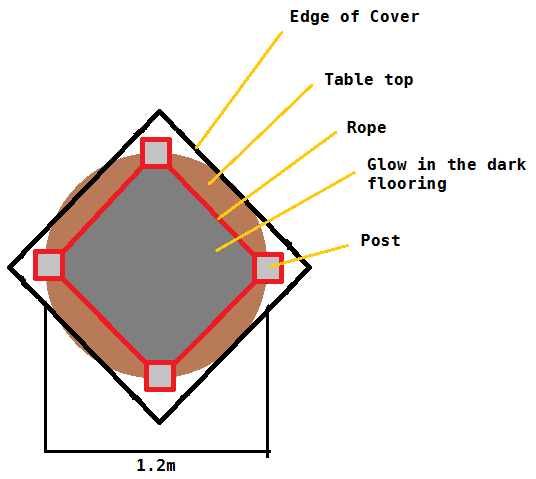
\includegraphics[scale=0.7]{img/ArenaTopDown.png}
  \caption{Top down view of the proposed dark room} \label{desSysTopImg}
\end{figure}
\begin{figure}
  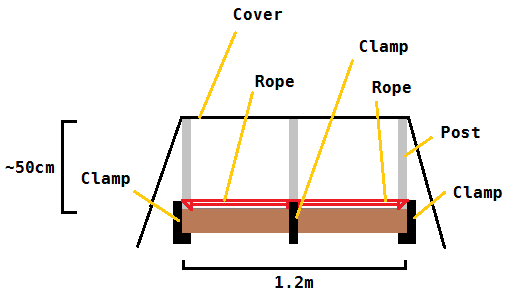
\includegraphics[scale=0.7]{img/ArenaSideView.png}
  \caption{Side view of the proposed dark room} \label{desSysSideImg}
\end{figure}
\clearpage

\subsection{Arena Design}
The design above is based on two main concepts -- flexibility and ease of use.
Once the glow in the dark flooring is placed, four posts are then clamped to the
edges of the table.  This ensures the flooring does not move and provides
stability for the rope.  Using a sheepshank knot, applied to the inner edges of
the posts as suggested in the top down view(\ref{desSysTopImg} ), it is 
estimated that to completely fence the arena with one piece of rope it should
approximately be 11 metres.  Using rope means that the arena can be of whatever
size is deemed appropriate, so long as there is enough to sufficiently cover the
generated edges.

Assuming a circular table, four posts, a sheepshank knot and wrapping the rope
around each post twice, the following algorithm calculates the minimum required
length of rope (it is suggested that you round up to the nearest half a metre 
to make sure):

\begin{algorithm}
  \caption{Rope Length Calculator (Measurements in centimetres) }
  \label{desSysRope}
  \begin{algorithmic}[1]
    \State $ Edge = 3(\sqrt{2(r^{2} ) } ) + 2 $
    \Comment Multiplying by 3 is due to tripling the rope over
    \State $ WrappedPost = (postPerimeter \times 2) + 2 $
    \Comment Trailing 2's are for securing the rope
    \State $ TotalRequiredRope = 4(Edge + WrappedPost) $
  \end{algorithmic}
\end{algorithm}